\begin{minipage}[c]{\textwidth}
\advance\leftskip-2.5cm
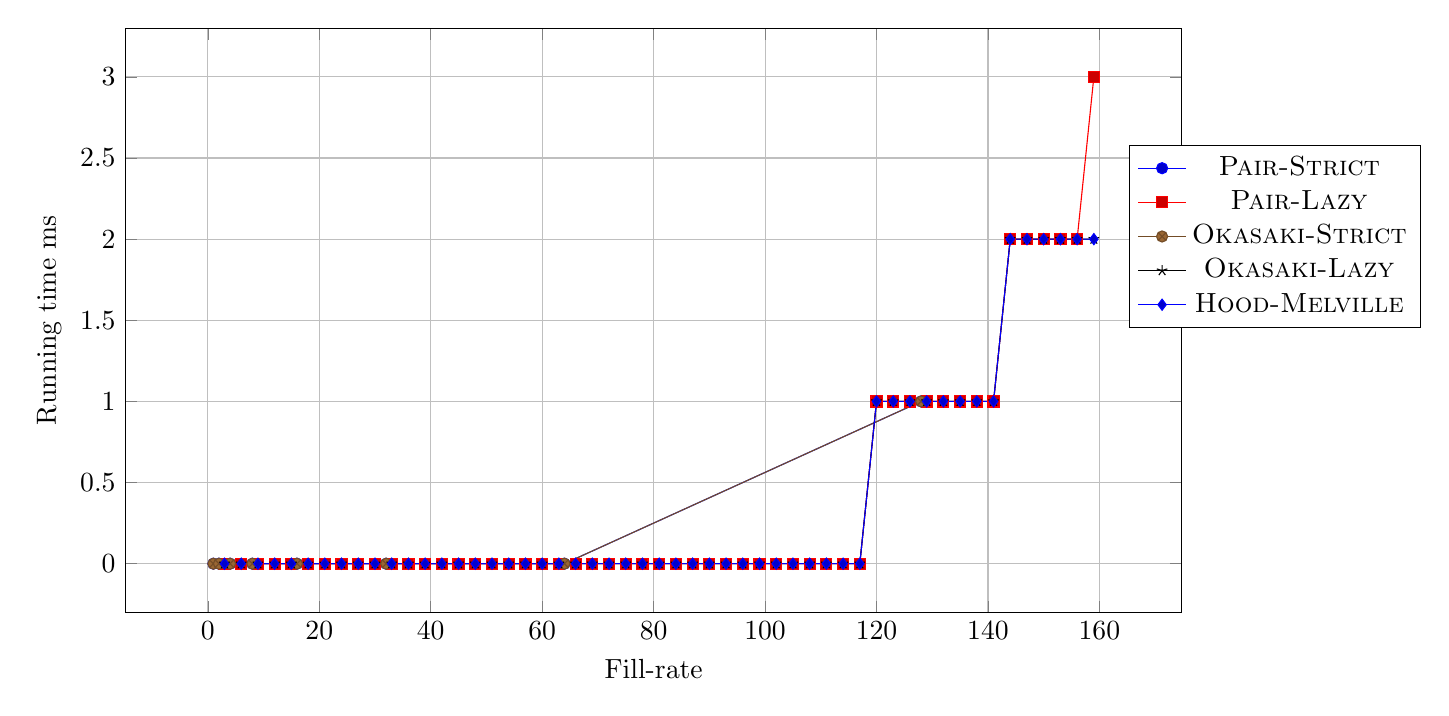
\begin{tikzpicture}
        \begin{axis}[
            xlabel = Fill-rate,
            ylabel = Running time ms,
            height=9cm,
            width=15cm,
            grid=major,
            legend style={
            at={(0.95,0.8)},
            anchor=north west}]            
            legend pos=center west
    	]
    		
  
                \addplot coordinates {
(1,0)
(2,0)
(4,0)
(8,0)
(16,0)
(32,0)
(64,0)
(128,1)

    	};
        
    	\addlegendentry{\textsc{Pair-Strict}}

        \addplot coordinates {
(3,0)
(6,0)
(9,0)
(12,0)
(15,0)
(18,0)
(21,0)
(24,0)
(27,0)
(30,0)
(33,0)
(36,0)
(39,0)
(42,0)
(45,0)
(48,0)
(51,0)
(54,0)
(57,0)
(60,0)
(63,0)
(66,0)
(69,0)
(72,0)
(75,0)
(78,0)
(81,0)
(84,0)
(87,0)
(90,0)
(93,0)
(96,0)
(99,0)
(102,0)
(105,0)
(108,0)
(111,0)
(114,0)
(117,0)
(120,1)
(123,1)
(126,1)
(129,1)
(132,1)
(135,1)
(138,1)
(141,1)
(144,2)
(147,2)
(150,2)
(153,2)
(156,2)
(159,3)

    	};
        
    	\addlegendentry{\textsc{Pair-Lazy}}

        \addplot coordinates {
(1,0)
(2,0)
(4,0)
(8,0)
(16,0)
(32,0)
(64,0)
(128,1)

    	};
        
    	\addlegendentry{\textsc{Okasaki-Strict}}

        \addplot coordinates {
(3,0)
(6,0)
(9,0)
(12,0)
(15,0)
(18,0)
(21,0)
(24,0)
(27,0)
(30,0)
(33,0)
(36,0)
(39,0)
(42,0)
(45,0)
(48,0)
(51,0)
(54,0)
(57,0)
(60,0)
(63,0)
(66,0)
(69,0)
(72,0)
(75,0)
(78,0)
(81,0)
(84,0)
(87,0)
(90,0)
(93,0)
(96,0)
(99,0)
(102,0)
(105,0)
(108,0)
(111,0)
(114,0)
(117,0)
(120,1)
(123,1)
(126,1)
(129,1)
(132,1)
(135,1)
(138,1)
(141,1)
(144,2)
(147,2)
(150,2)
(153,2)
(156,2)
(159,2)

    	};
        
    	\addlegendentry{\textsc{Okasaki-Lazy}}

        \addplot coordinates {
(3,0)
(6,0)
(9,0)
(12,0)
(15,0)
(18,0)
(21,0)
(24,0)
(27,0)
(30,0)
(33,0)
(36,0)
(39,0)
(42,0)
(45,0)
(48,0)
(51,0)
(54,0)
(57,0)
(60,0)
(63,0)
(66,0)
(69,0)
(72,0)
(75,0)
(78,0)
(81,0)
(84,0)
(87,0)
(90,0)
(93,0)
(96,0)
(99,0)
(102,0)
(105,0)
(108,0)
(111,0)
(114,0)
(117,0)
(120,1)
(123,1)
(126,1)
(129,1)
(132,1)
(135,1)
(138,1)
(141,1)
(144,2)
(147,2)
(150,2)
(153,2)
(156,2)
(159,2)

    	};

    	\addlegendentry{\textsc{Hood-Melville}}

        \end{axis}

    \end{tikzpicture}
    \captionof{figure}{TITEL}
    \label{fig:sample_figure}
\end{minipage}